\section{Session 5 - Sequential circuit and unit}
\vspace{-15pt}\noindent\rule{\textwidth}{0.1pt}\vspace{-10pt}
    \subsection{Notes}
    {\color{hwSolution}
    \subsection*{Another method to generate delayed paluse - without losing its length}
        \begin{center}\begin{tikzpicture}
% CHIP 2 (Y+0.0)
  \draw[black,thick]
    (-1.2,2.4)--(-1.2,0.0)
  --( 1.2,0.0)--( 1.2,2.4)
  --cycle;
  % Left Side
  \draw[black,thick, -] (-1.2,1.6) node[right]{$A$}
  -- (-2.0,1.6) node[left]{$V_{DD}$};
  \draw[black,thick,o-] (-1.2, 0.8) node[right]{$B$}
  -- (-2.0,0.8);
  % Right Side
  \draw[black,thick, -] ( 1.2, 1.6) node[left]{$Q$}
  -- ( 2.0, 1.6);
  \draw[black,thick,o-] ( 1.2, 0.8) node[left]{$\bar{Q}$}
  -- ( 1.4, 0.8);
  % Top Side
  \draw[black,thick, -] (-0.4, 2.4) node[below]{$C_X$}
  -- (-0.4, 3.0);
  \draw[black,thick, -] ( 0.4, 2.4) node[below]{$R_X$}
  -- ( 0.4, 3.0);
  % Bottom Side
  \draw[black,thick,o-*] ( 0.0, 0.0) node[above]{$C_{L}$}
  -- ( 0.0,-0.6) -- ( 1.8,-0.6);
  % C/R
  \draw[black,thick, -]
      % Capacitor
      (-0.4, 3.0) -- (-0.1, 3.0)
      ( 0.4, 3.0) -- ( 0.1, 3.0)
      ( 0.1, 3.2) -- ( 0.1, 2.8)
      (-0.1, 3.2) -- (-0.1, 2.8)
      ( 0.0, 3.2) node[above]{$C$}
      % Resistor
      ( 0.4, 3.0) -- ( 0.7, 3.0)
      ( 1.2, 3.0) -- ( 1.5, 3.0)
      ( 0.7, 3.1) -- ( 1.2, 3.1) -- ( 1.2, 2.9) -- ( 0.7, 2.9) -- cycle
      ( 0.95, 3.2) node[above]{$R$};
  \draw[black,thick,-*] ( 1.5, 3.0) -- ( 1.8, 3.0);
% CHIP 1 (Y+5.0)
    \draw[black,thick]
    (-1.2,7.4)--(-1.2,5.0)
  --( 1.2,5.0)--( 1.2,7.4)
  --cycle;
  % Left Side
  \draw[black,thick, -] (-1.2,6.6) node[right]{$A$}
  -- (-2.0,6.6);
  \draw[black,thick,o-] (-1.2, 5.8) node[right]{$B$}
  -- (-2.0,5.8) node[left]{\textit{GND}};
  % Right Side
  \draw[black,thick, -] ( 1.2, 6.6) node[left]{$Q$}
  -- ( 2.0, 6.6);
  \draw[black,thick,o-] ( 1.2, 5.8) node[left]{$\bar{Q}$}
  -- ( 1.4, 5.8);
  % Top Side
  \draw[black,thick, -] (-0.4, 7.4) node[below]{$C_X$}
  -- (-0.4, 8.0);
  \draw[black,thick, -] ( 0.4, 7.4) node[below]{$R_X$}
  -- ( 0.4, 8.0);
  % Bottom Side
  \draw[black,thick,o-*] ( 0.0, 5.0) node[above]{$C_{L}$}
  -- ( 0.0, 4.4) -- ( 1.8, 4.4);
  % C/R
  \draw[black,thick, -]
    % Capacitor
    (-0.4, 8.0) -- (-0.1, 8.0)
    ( 0.4, 8.0) -- ( 0.1, 8.0)
    ( 0.1, 8.2) -- ( 0.1, 7.8)
    (-0.1, 8.2) -- (-0.1, 7.8)
    ( 0.0, 8.2) node[above]{$C$}
    % Resistor
    ( 0.4, 8.0) -- ( 0.7, 8.0)
    ( 1.2, 8.0) -- ( 1.5, 8.0)
    ( 0.7, 8.1) -- ( 1.2, 8.1) -- ( 1.2, 7.9) -- ( 0.7, 7.9) -- cycle
    ( 0.95,8.2) node[above]{$R$};
  \draw[black,thick,-*] ( 1.5, 8.0) -- ( 1.8, 8.0);
% AND Gate (4.0,3.7)
  \draw[black,thick]
  (4.0,3.7) node{$\&$}
  (3.5,2.9)--(3.5,4.5)
  --(4.5,4.5)--(4.5,2.9)
  --cycle;
% Wire
  \draw[black,thick, -] ( 1.7, 9.0) node[above]{$V_{DD}$}
  -- ( 1.7,-0.6);
  \draw[black,thick, -] (-6.0, 3.7) node[left]{$D_{IN}$} -- (-4.0, 3.7)
  -- (-4.0,6.6) -- (-2.0,6.6)
  (-4.0, 3.7) -- (-4.0,0.8) -- (-2.0,0.8);
  \draw[black,thick, -]
  ( 2.0, 1.6) -- ( 3.0, 1.6) -- ( 3.0, 3.4) -- ( 3.5, 3.4)
  ( 2.0, 6.6) -- ( 3.0, 6.6) -- ( 3.0, 4.0) -- ( 3.5, 4.0);
  \draw[black,thick, -] (4.5,3.7) -- (6.0,3.7) node[right]{$D_{OUT}$};
\end{tikzpicture}\end{center}

        Functionality analysis:

        \begin{center}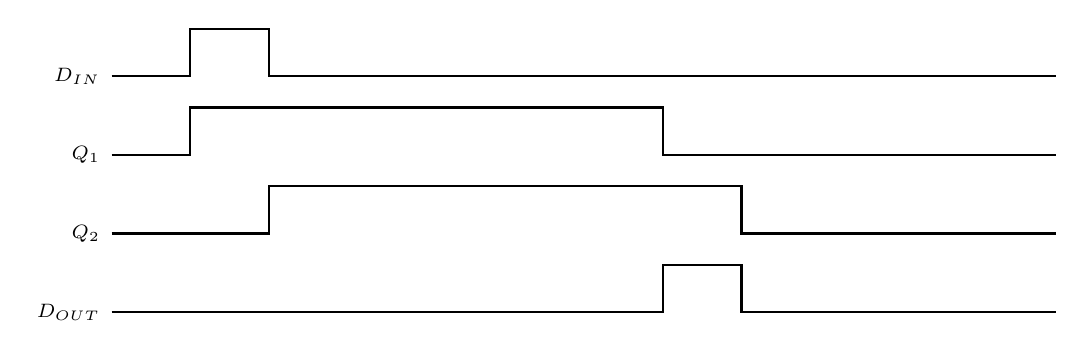
\begin{tikzpicture}
            \draw[black,thick]
                (0.0,3.0) node[left]{$_{D_{IN}}$}
                --(0.0,3.0)
                --(1.0,3.0)--(1.0,3.6)
                --(2.0,3.6)--(2.0,3.0)
                --(12.0,3.0);
            \draw[black,thick]
                (0.0,2.0) node[left]{$_{Q_{1}}$}
                --(0.0,2.0)
                --(1.0,2.0)--(1.0,2.6)
                --(7.0,2.6)--(7.0,2.0)
                --(12.0,2.0);
            \draw[black,thick]
                (0.0,1.0) node[left]{$_{Q_{2}}$}
                --(0.0,1.0)
                --(2.0,1.0)--(2.0,1.6)
                --(8.0,1.6)--(8.0,1.0)
                --(12.0,1.0);
            \draw[black,thick]
                (0.0,0.0) node[left]{$_{D_{OUT}}$}
                --(0.0,0.0)
                --(7.0,0.0)--(7.0,0.6)
                --(8.0,0.6)--(8.0,0.0)
                --(12.0,0.0);
        \end{tikzpicture}\end{center}
    }
    \subsection{Homework}
    \subsubsection{8.3 \textnormal{Analyze Logical function of the given circuit}.}
        \begin{center}\begin{tikzpicture}
    \draw[black,thick,->] (-0.5,0) -- (10,0) node[below]{$t$};
    \draw[black,thick,->] (0,-0.5) -- ( 0,3.5) node[left]{$u_I$};
    \draw[black,dash pattern={on 0.2cm off 0.2cm}]
    (0,1) node[left]{$U_{T-}$} -- (9.5,1)
    (0,2) node[left]{$U_{T+}$} -- (9.5,2);
    \draw[gray,thick] plot[smooth] coordinates{
    (0,0)
    (0.5,2.0) %N1
    (0.7,2.2)
    (1.1,1.8)
    (1.4,2.1)
    (1.6,1.8)
    (1.9,2.1)
    (2.2,1.0) %N2
    (2.3,0.0)
    (2.8,1.0)
    (3.0,1.3)
    (3.3,1.4)
    (3.5,0.8)
    (3.7,1.2)
    (4.1,0.7)
    (4.6,2.0) %N3
    (5.1,2.3)
    (5.3,1.8)
    (5.5,1.8)
    (5.9,2.6)
    (6.2,1.0) %N4
    (6.6,0.0)
    (7.0,1.3)
    (7.6,0.8)
    (7.9,1.3)
    (8.4,0.8)
    (9.0,1.2)};
    \draw[hwSolution,thick](0,0.5) node[left,hwSolution]{$u_0$}
    -- (0.5,0.5) -- (0.5,2.5)
    -- (2.2,2.5) -- (2.2,0.5)
    -- (4.6,0.5) -- (4.6,2.5)
    -- (6.2,2.5) -- (6.2,0.5)
    -- (9.0,0.5);
\end{tikzpicture}\end{center}
    {\color{hwSolution}
        
    }
 
    \subsubsection{8.6 \textnormal{}.}
    {\color{hwSolution}

    }

    \subsubsection{8.7 \textnormal{}.}
    {\color{hwSolution}
  
    }

    \subsubsection{8.12 \textnormal{}.}
    {\color{hwSolution}

    }

    \subsubsection{8.13 \textnormal{}.}
    {\color{hwSolution}

    }

    \subsubsection{8.17 \textnormal{}.}
    {\color{hwSolution}

    }